% latex article template

% cheat sheet(eng): http://www.pvv.ntnu.no/~walle/latex/dokumentasjon/latexsheet.pdf
% cheat sheet2(eng): http://www.pvv.ntnu.no/~walle/latex/dokumentasjon/LaTeX-cheat-sheet.pdf
% reference manual(eng): http://ctan.uib.no/info/latex2e-help-texinfo/latex2e.html

% The document class defines the type of document. Presentation, article, letter, etc. 
\documentclass[12pt, a4paper]{article}

% packages to be used. needed to use images and such things. 
\usepackage[pdfborder=0 0 0]{hyperref}
\usepackage[utf8]{inputenc}
\usepackage[english]{babel}
\usepackage{graphicx}
\PassOptionsToPackage{hyphens}{url}

% hides the section numbering. 
\setcounter{secnumdepth}{-1}

% Graphics/image lications and extensions. 
\DeclareGraphicsExtensions{.pdf, .png, .jpg, .jpeg}
\graphicspath{{./images/}}

% Title or header for the document. 
\title{
	TIØ4116, Exercise 11. 
}
% Author
\author{
	Magnus L. Kirø \\
}
\date{\today}

\begin{document}
\maketitle
\pagenumbering{arabic}

\section{Task 1}
demand: B(n), for n=1...N,
travel cost: t(n)= fuel+time(n),
total cost: T(n)=n*t(n),

\paragraph{A}
While n0 is larger than n we get a negative number of the second part of the
cost function. We cannot have negative cost and therefore eliminates all
negative possibilities by saying that the cost is fixed at n=0.  

\paragraph{B}
When n increases with 1, the additional cost for all cars are:
((n+1)-n_{0})^2)n

\paragraph{C}
By plotting the significant part of the cost function we get a parabola.
Interpreting the parabola we can see that increased traffic gives exponential
increase in costs. But as we don't know anything about the capacity of the
road, or the size of the minimum cost. And we cannot say anything about the
practical value of 1 money in this case. 

% image example. 
\begin{figure}[htb]
    \centering
    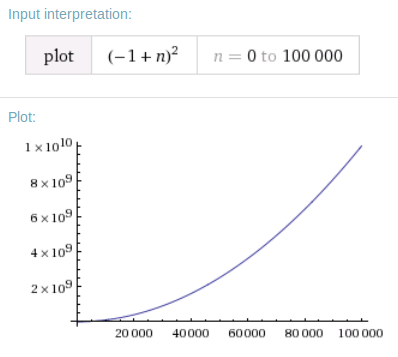
\includegraphics[width=\textwidth]{plot} 
    \label{fig:plot}
The figure shows the increase in cost per car given the amount of other cars on
the road. 
\end{figure}

\section{Task 2}
\paragraph{A}
1: 20mill in values. 2: minus 10 mill in values. 

The chance of getting either is 0.5. Then the sales value now will be estimated
to 20-10=10. The expected max return minus the expected minimum return gives us
the average expected return. Which can be seen as the expected sales value. 

\paragraph{B}
Guaranteed government backing. The minimum of value of the company is zero.
Which in turn increases the expected value of the company to 20 mill. 

The government still have to expect to pay 10 million, as that is the
guaranteed amount. Debt goes down, shares goes up. 

\paragraph{C}
If the 80\% debt is converted to shares the perceived value of the company is
increased to 100 mill. 

\paragraph{D}
When the loans are converted to shares and the loaners collect interest the
value of the original share decrease. 

\paragraph{E}
Converting the debt into shares without government backing does not change the
value of the company.

\paragraph{F}

\section{Task 3}
\paragraph{A}
The director should choose the 120 share value. This gives the best potential
for reward. 

\paragraph{B}
The director will choose options. Options is the safer choice for long term
investments in this case. 

\paragraph{C}

\end{document}
This is never printed
